
% ===============================================================================================
% ===============================================================================================
% INTRODUCTION
% 
% Small introduction tale : how to make lots of sandwiches ?
%
% ===============================================================================================
% ===============================================================================================

\subsection{Introduction}

\begin{frame}[containsverbatim]
\frametitle{}
\begin{center}
\textbf{Let's go PARALLEL !!}
\end{center}
\end{frame}

\begin{frame}[containsverbatim]
\frametitle{Introductory tale}
\begin{center}
        {
\includegraphics[height=2.5cm]{Day0/images/gateau.png}}
\end{center}
\begin{center}
Next wednesday afternoon, it's Charlotte's 10$^{th}$ birthday party ! She decides to invite 20 friends.
\end{center}
\end{frame}

\begin{frame}[containsverbatim]
\frametitle{Introductory tale}
\begin{center}
        {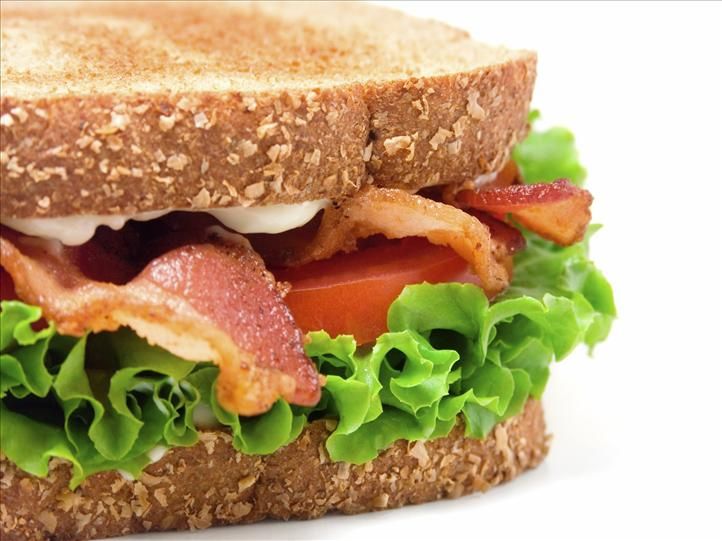
\includegraphics[height=2.5cm]{Day0/images/sandwich.jpg}}
\end{center}
\begin{center}
... Mrs. Smith -- her mother -- will not cook special things. All the family will prepare sandwiches for Charlotte's friends. Daddy Smith and Charlotte's brother -- Mike -- too... 
\end{center}
\end{frame}


\begin{frame}[containsverbatim]
\frametitle{Introductory tale}
\begin{center}
        {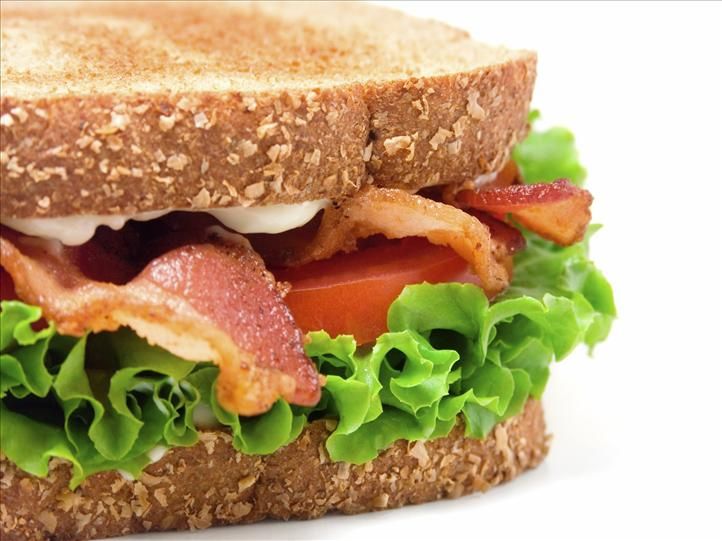
\includegraphics[height=2.5cm]{Day0/images/sandwich.jpg}}
\end{center}
\begin{center}
... Mrs. Smith knows how to make a sandwich for many years. Four steps of approximatively the same duration (1 unit of time) are required :
\begin{enumerate}
	\item{\textbf{cut the bread in two halves}}
	\item{\textbf{spread the butter on the bread}}
	\item{\textbf{add a piece of ham/cheese, a few pickles and some mustard }}
	\item{\textbf{close the sandwich carefully and put it on a tray}}
\end{enumerate}
\end{center}

\end{frame}


\begin{frame}[containsverbatim]
\frametitle{Introductory tale}
\begin{center}
        {
\includegraphics[height=2.5cm]{Day0/images/interrogation.png}}
\end{center}
\begin{center}
... how the family could proceed to produce 20 sandwiches in the more efficient manner ...
\end{center}

\end{frame}



\begin{frame}[containsverbatim]
\frametitle{Introductory tale}
\begin{center}
        {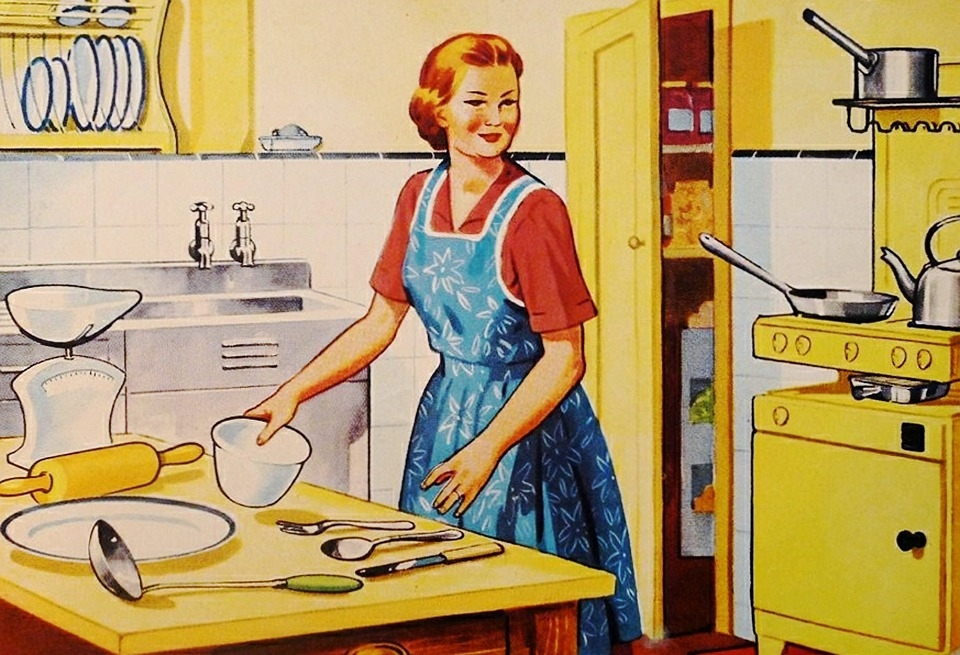
\includegraphics[height=2.5cm]{Day0/images/oldschool.jpg}}
\end{center}
\begin{center}
... old-school fashion ? Mrs. Smith does it all alone while Mr. Smith and kids watch TV ? 
\end{center}
\begin{center}
\begin{itemize}
	\item{\textbf{Pros: }
		\begin{itemize}
			\item{Mrs. Smith does it well without having to explain to non-professionals}
		\end{itemize}
	}
	\item{\textbf{Cons: }
		\begin{itemize}
			\item{What happens if Charlotte decides to invite the whole school to her birthday party ?}
		\end{itemize}
	}
\end{itemize}
\textbf{Time to make 20 sandwiches = 80 units of time}
\end{center}
\end{frame}


\begin{frame}[containsverbatim]
\frametitle{Introductory tale}
\begin{center}
        {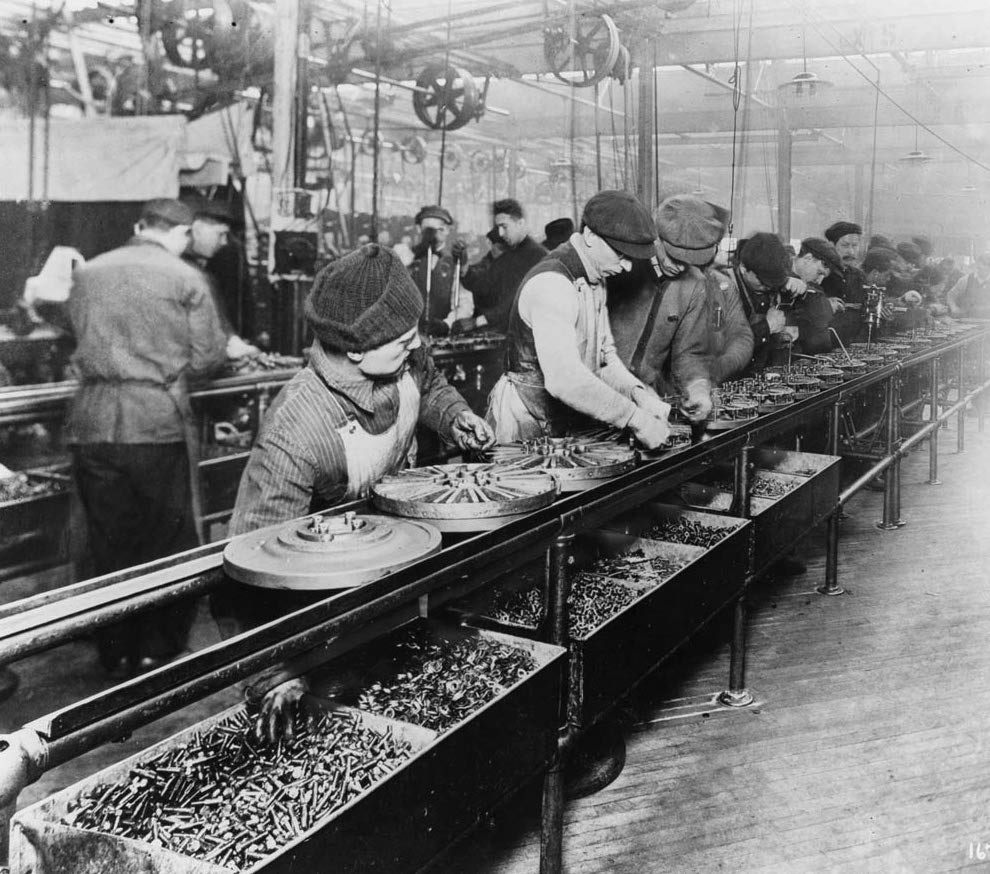
\includegraphics[height=2.5cm]{Day0/images/ford.jpg}}
\end{center}
\begin{center}
... 1923 Ford T mode ? Mrs Smith cuts the bread, then Mr. Smith spread the butter while Mrs. Smith cuts a new bread, Charlotte adds ham and pickles while Mrs. cuts a bread finally Mike closes the sandwich and put it in a tray.
\end{center}
\begin{center}
\begin{itemize}
	\item{\textbf{Pros: }
		\begin{itemize}
			\item{4x more sandwiches produced when the pipeline is full}
			\item{specialized tasks, very few communications}
		\end{itemize}
	}
	\item{\textbf{Cons: }
		\begin{itemize}
			\item{each step must have the same duration}
			\item{No place for Shirley (Charlotte's best friend). 4 friends are required to produce 8x more sandwiches}
		\end{itemize}
	}
\end{itemize}
\textbf{Time to make 20 sandwiches = 23 units of time}
\end{center}
\end{frame}

\begin{frame}[containsverbatim]
\frametitle{Introductory tale}
\begin{center}
        {
\includegraphics[height=2.5cm]{Day0/images/fourmis.png}}
\end{center}
\begin{center}
... totally distributed ? Mrs. \& Mr. Smith, Charlotte and Mike produce 5 sandwiches each ...
\end{center}
\begin{center}
\begin{itemize}
	\item{\textbf{Pros: }
		\begin{itemize}
			\item{Most efficient solution : number of sandwiches to produce / number of people}
		\end{itemize}
	}
	\item{\textbf{Cons: }
		\begin{itemize}
			\item{resources problem : need for 4 knives, 4 portions of butter, 4 portions of ham, etc..}
			\item{deadlocks : if only 1 knife is available, one person works when the other wait}
		\end{itemize}
	}
\end{itemize}
\textbf{Time to make 20 sandwiches = 20 units of time}
\end{center}
\end{frame}


